\chapter{Visão Geral}

Para embasar e planejar o projeto a ser desenvolvido, uma proposta de
arquitetura precisa ser feito. Neste capítulo será apresentado a proposta do projeto UMISS,
sendo explanado as arquiteturas de cada subsistema.

\section{Subsistema - Processamento de Sinais e Monitoramento}

O subsistema de controle e monitoramento terá como grande objetivo a aquisição
dos sinais do paciente, a disponibilização desses recursos para os
interessados, e a notificação dos responsáveis em casos de eventos críticos.
Sua arquitetura pode ser dividido em três grandes
módulos: o módulo que chamaremos \textbf{módulo eletrônico}, que conterá
grande parte dos componentes eletrônicos do projeto,
o \textbf{módulo servidor remoto}, que será um servidor remoto disponível
para ser consumido por outros serviços, e o \textbf{módulo aplicativo},
que será uma solução em aplicativo para ser utilizado pelos interessados.

\subsection{Módulo Eletrônico}
O módulo eletrônico será composto principalmente por sensores, amplificadores,
filtros, conversores, e um sistema embarcado.

Os sensores terão como principal papel a extração dos sinais vitais do
paciente, e serão acoplados a estrutura da cadeira, de forma que algum
membro do paciente fique em contato com o sensor, permitindo assim a
aquisição do sinal.

Os amplificadores e filtros serão responsáveis pelo tratamento do sinal;
amplificadores tendo o papel de aumentar o ganho extraído pelo sinal,
e os filtros tendo o papel de atenuar ruídos capturados.

Os conversores terão como papel a conversão dos sinais tratados para um formato
que o sistema embarcado possa entender; no caso do projeto UMISS, a conversão
a ser feita será de analógica para digital.

Um sistema embarcado será responsável por receber os sinais do paciente,
processá-los e utilizá-los em tarefas específicas, e, por fim, despachar os
dados para o módulo servidor remoto.

\subsection{Módulo Servidor Remoto}
O módulo servidor remoto é dividido nos seguintes componentes: um servidor remoto
e gerência de configuração do servidor.

O servidor remoto será um servidor hospedado fora da rede-interna da parte
eletrônica, e poderá ser acessado via \textit{internet}. Se comunicará com
o sistema embarcado da parte eletrônica utilizando comunicação
\textit{via socket}\footnote{\url{https://docs.oracle.com/javase/tutorial/networking/sockets/definition.html}},
apresentará dados para o aplicativo, e o notificará da ocorrência de eventos
críticos.

A gerência de configuração do servidor será composta principalmente de
configurações e \textit{scripts} que vão permitir a manutenção e
interoperabilidade entre o servidor e outros recursos.

\subsection{Módulo aplicativo}

O aplicativo só tem si próprio como componente, e será utilizado regularmente
pelos responsáveis do paciente; estará preparado para receber as notificações
do servidor e para mostrar os dados em tempo real.

\subsection{Integração entre os módulos}

\begin{figure}[H]
  \centering
    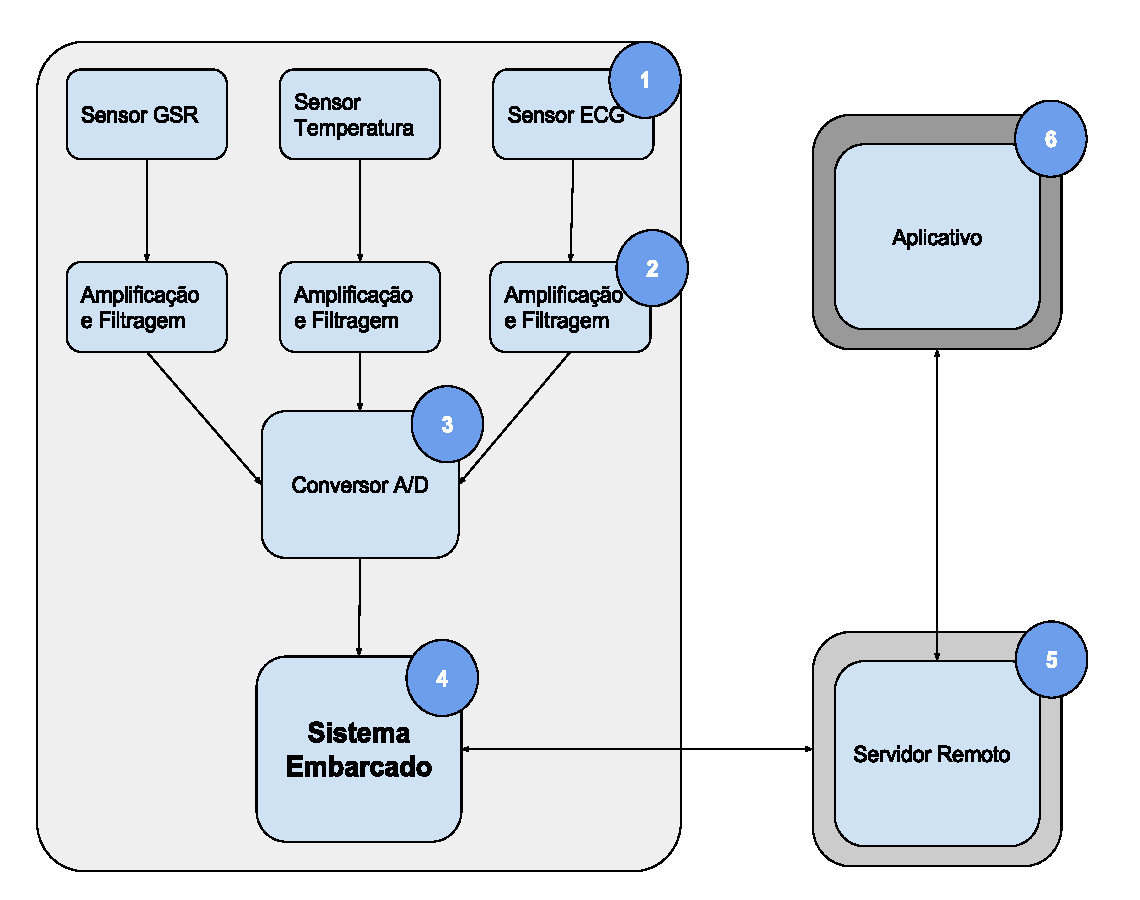
\includegraphics[width=\textwidth]{figuras/arquitetura-monitoramentoecontrole.eps}
  \caption{Fluxo típico do subsistema de Monitoramento e Controle}
  \label{fig:arquitetura-monitoramento-e-controle}
\end{figure}

O passo (1) do subsistema é atuado pelos sensores, que extraírão sinais do paciente;
o passo (2) será atuado pelos amplificadores e filtros, e tratarão o sinal
extraído pelos sensores no passo anterior; no passo (3) os sinais tratados
são convertidos para formato digital, para que possam ser lidos pelo sistema
embarcado; no passo (4) o sistema embarcado recebe as informações do conversor
e abre conexão com o servidor remoto - após, envia as informações recebidas,
quando necessário; no passo (5) o servidor remoto recebe dados do sistema
embarcado e passa informações importantes para o aplicativo, e, por fim,
no passo (6), o aplicativo recebe as informações.

\subsection{Tecnologias Utilizadas}

\subsubsection{Servidor Django}
\label{sub:servidor_django}
O passo (5), retratado na Figura \ref{fig:arquitetura-monitoramento-e-controle},
representa o servidor remoto, que irá receber as informações de todas as
estações embarcadas do sistema. Este será responsável por receber, processar
e se comunicar com os dispositivos móveis cadastrados no sistema. Para tal,
será utilizado uma linguagem de programação compatível com a que será utilizada
no software embarcado, que será escrito em python. Desta maneira, todo
o servidor proverá serviços utilizando python.

Um Framework robusto e já bastante consolidado na comunidade python é o Django.
Este é bem completo e possui várias ferramentas que auxiliam no desenvolvimento.
O django possui um framework para API's Rest, que será o padrão utilizado pelos
clientes para se comunicarem, chamado de DjangoRestFramework. Este é muito poderoso
e de alta produtividade.

Estas três ferramentas irão compor juntas o passo (5).

\section{Subsistema - Controle e Alimentação}

\section{Subsistema - Projeto Estrutural}

\section{Outros}

\subsection{Integração Contínua}
